\PassOptionsToPackage{unicode}{hyperref}
\PassOptionsToPackage{hyphens}{url}
\documentclass[
]{article}
\usepackage{lmodern}
\usepackage{amssymb,amsmath}
\usepackage{ifxetex,ifluatex}
\ifnum 0\ifxetex 1\fi\ifluatex 1\fi=0 % if pdftex
  \usepackage[T1]{fontenc}
  \usepackage[utf8]{inputenc}
  \usepackage{textcomp} % provide euro and other symbols
\else % if luatex or xetex
  \usepackage{unicode-math}
  \usepackage{hyperref}
  \usepackage{verbatim}
  \defaultfontfeatures{Scale=MatchLowercase}
  \defaultfontfeatures[\rmfamily]{Ligatures=TeX,Scale=1}
\fi
% Use upquote if available, for straight quotes in verbatim environments
\IfFileExists{upquote.sty}{\usepackage{upquote}}{}
\IfFileExists{microtype.sty}{% use microtype if available
  \usepackage[]{microtype}
  \UseMicrotypeSet[protrusion]{basicmath} % disable protrusion for tt fonts
}{}
\makeatletter
\@ifundefined{KOMAClassName}{% if non-KOMA class
  \IfFileExists{parskip.sty}{%
    \usepackage{parskip}
  }{% else
    \setlength{\parindent}{0pt}
    \setlength{\parskip}{6pt plus 2pt minus 1pt}}
}{% if KOMA class
  \KOMAoptions{parskip=half}}
\makeatother
\usepackage{xcolor}
\IfFileExists{xurl.sty}{\usepackage{xurl}}{} % add URL line breaks if available
\IfFileExists{bookmark.sty}{\usepackage{bookmark}}{\usepackage{hyperref}}
\hypersetup{
  hidelinks,
  pdfcreator={LaTeX via pandoc}}
\urlstyle{same} % disable monospaced font for URLs
\usepackage{graphicx}
\makeatletter
\def\maxwidth{\ifdim\Gin@nat@width>\linewidth\linewidth\else\Gin@nat@width\fi}
\def\maxheight{\ifdim\Gin@nat@height>\textheight\textheight\else\Gin@nat@height\fi}
\makeatother
% Scale images if necessary, so that they will not overflow the page
% margins by default, and it is still possible to overwrite the defaults
% using explicit options in \includegraphics[width, height, ...]{}
\setkeys{Gin}{width=\maxwidth,height=\maxheight,keepaspectratio}
% Set default figure placement to htbp
\makeatletter
\def\fps@figure{htbp}
\makeatother
\setlength{\emergencystretch}{3em} % prevent overfull lines
\providecommand{\tightlist}{%
  \setlength{\itemsep}{0pt}\setlength{\parskip}{0pt}}
\setcounter{secnumdepth}{-\maxdimen} % remove section numbering

\author{Duong Tung}
\date{\today}

\begin{document}
\begin{center}

    \textbf{Student name:} Duong Doan Tung\\

    \textbf{Student ID:} 21010294\\
    \textbf{Course:} Applied Mathematics for Artificial Intelligence\\

\end{center}

Google colab notebook contains all the Python solution code for this assignment.\\
\textbf{Hyper link to google colab notebook: }\href{https://colab.research.google.com/github/dtungpka/Applied-Mathematics-for-Artificial-Intelligence/blob/main/Assignment_3/Assignment%203.ipynb}{Assignment 3.ipynb}\\
Problem 1:

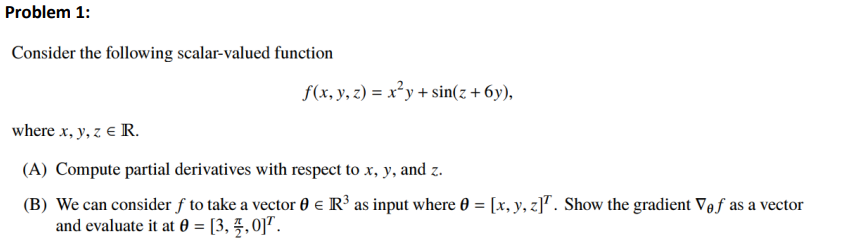
\includegraphics[width=6.52349in,height=1.70833in]{image1.png}




(A)

\[{f\ '}_{x} = 2xy\]

\[{f\ '}_{y} = x^{2} + 6cos(z + 6y)\]

\[{f\ '}_{z} = cos(z + 6y)\]

\emph{(B)}

\[\nabla_{\theta}f = \left\lbrack 2xy,x^{2} + 6cos(z + 6y),cos(z + 6y)\  \right\rbrack^{T}\]

Where
\(\theta = \left\lbrack 3,\frac{\pi}{2},0 \right\rbrack^{T} \Rightarrow \left\{ \begin{matrix}
    x = 3     \\
    y = \pi/2 \\
    z = 0     \\
\end{matrix} \right.\ \)

Therefore,
\(\nabla_{\theta}f = \left\lbrack 3\pi,3, - 1 \right\rbrack^{T}\)

\textbf{Code implementation:} \href{https://colab.research.google.com/github/dtungpka/Applied-Mathematics-for-Artificial-Intelligence/blob/main/Assignment_3/Assignment%203.ipynb#scrollTo=Problem_1}{Problem 1}


%insert page break
\newpage
Problem 2:

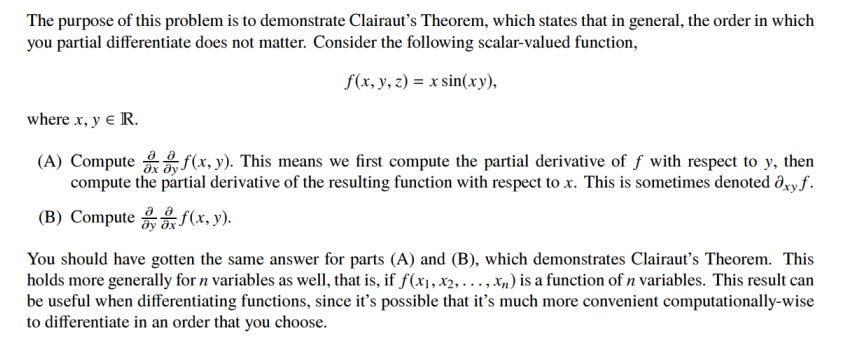
\includegraphics[width=6.49167in,height=1.84167in]{image2.png}

\emph{(A)}

\[\frac{\partial\ }{\partial y}f = x^{2}cos(xy) = > \frac{\partial\ }{\partial x}\frac{\partial\ }{\partial y}f = 2xcos(xy) - x^{2}ysin(xy)\]

\emph{(B)}

\[\frac{\partial}{\partial x}f = sin(xy) + xycos(xy) = > \frac{\partial\ }{\partial y}\frac{\partial\ f}{\partial x} = xcos(xy) + xcos(xy) - x^{2}ysin(xy)\]

\emph{=\textgreater{} Clairaut's Theorem is true for this function.}\\
\textbf{Code implementation:} \href{https://colab.research.google.com/github/dtungpka/Applied-Mathematics-for-Artificial-Intelligence/blob/main/Assignment_3/Assignment%203.ipynb#scrollTo=Problem_2}{Problem 2}

\newpage
\emph{Problem 3:}

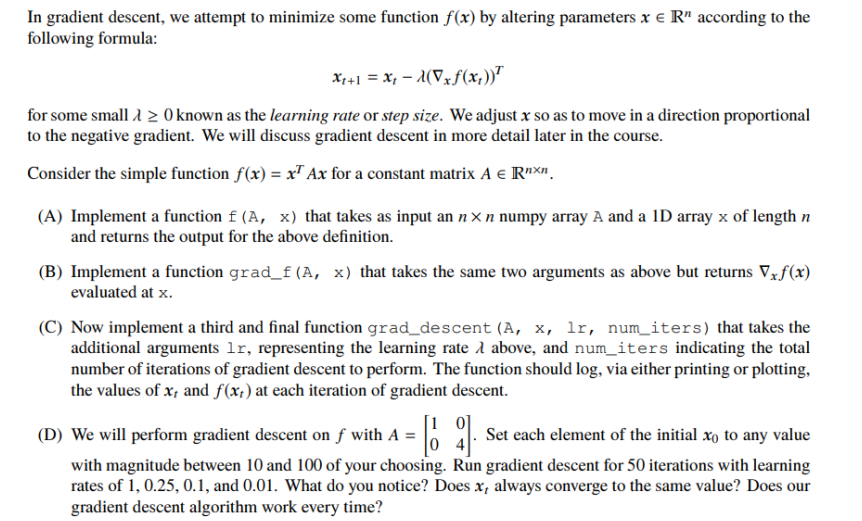
\includegraphics[width=6.49167in,height=2.74167in]{image3.png}
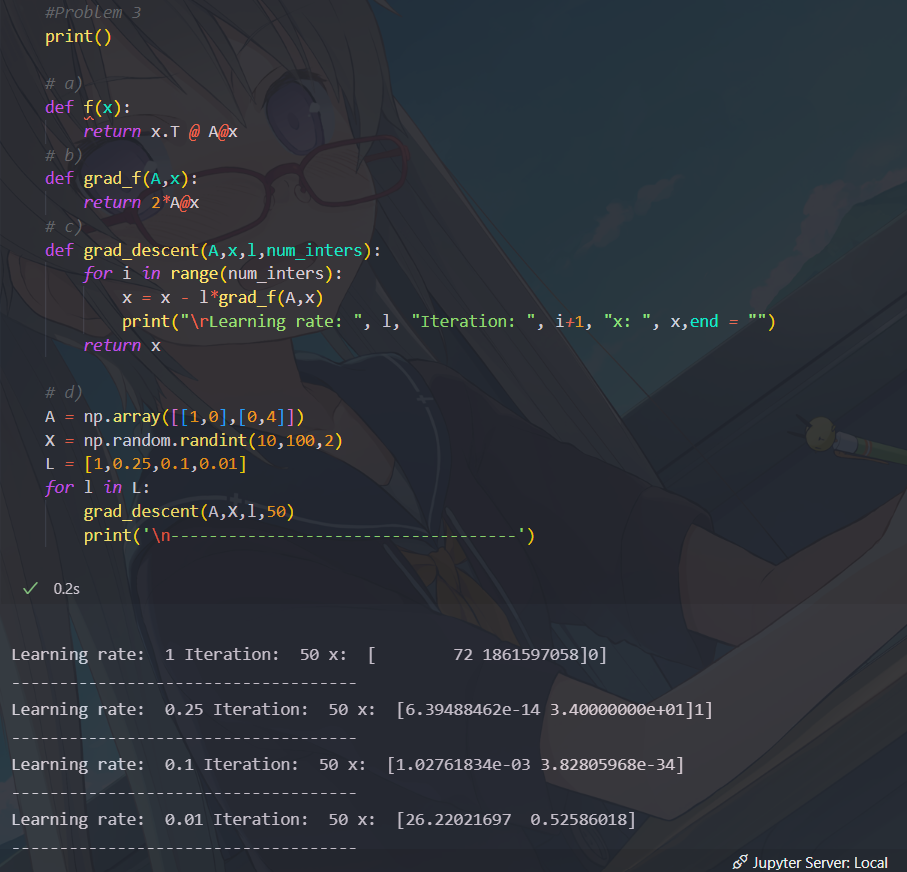
\includegraphics[width=6.49167in,height=4.24167in]{image4.png}
\textbf{Code implementation:} \href{https://colab.research.google.com/github/dtungpka/Applied-Mathematics-for-Artificial-Intelligence/blob/main/Assignment_3/Assignment%203.ipynb#scrollTo=Problem_3}{Problem 3}

\newpage
Problem 4:\\
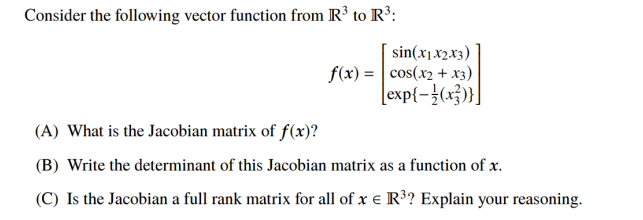
\includegraphics[width=6.49167in,height=1.84167in]{image5.png}\\
A)\\
\[J = \begin{bmatrix}
    \frac{\partial f(x)}{\partial x_{1}} & \frac{\partial f(x)}{\partial x_{2}} & \frac{\partial f(x)}{\partial x_{3}} \\
    \end{bmatrix} = \begin{bmatrix}
    x_{2}x_{3}\cos{(x_{1}x_{2}x_{3})} & x_{1}x_{3}\cos{(x_{1}x_{2}x_{3})} & x_{1}x_{2}\cos{(x_{1}x_{2}x_{3})} \\
    0 & - \sin{(x_{2}{+ x}_{3})} & - \sin{(x_{2}{+ x}_{3})} \\
    0 & 0 & - x_{3}e^{\frac{- 1}{2}({x_{3}}^{2})} \\
    \end{bmatrix}\]\\
    
    B) determinant of the Jacobian:
    
    \(\left| J \right| = \left( x_{2}x_{3}\cos\left( x_{1}x_{2}x_{3} \right) \right)*\)(\(- \sin{(x_{2}{+ x}_{3})}\))*(\(\  - x_{3}e^{\frac{- 1}{2}({x_{3}}^{2})}\))
    
    \[= x_{2}{x_{3}}^{2}{(e}^{\frac{- 1}{2}({x_{3}}^{2})})\cos\left( x_{1}x_{2}x_{3} \right)\sin{(x_{2}{+ x}_{3})}\]
    
   C)  This Jacobian is full rank for all of $x \in  R^{3} $ because the determinant is not equal to 0 for all $x \in R^{3}$.\\
   \textbf{Code implementation:} \href{https://colab.research.google.com/github/dtungpka/Applied-Mathematics-for-Artificial-Intelligence/blob/main/Assignment_3/Assignment%203.ipynb#scrollTo=Problem_4}{Problem 4}
\\ \newpage Problem 5:\\
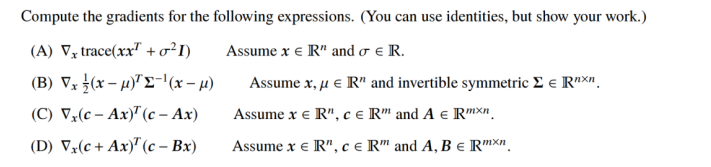
\includegraphics[width=6.49167in,height=1.84167in]{image8.png}\\



\emph{a)} \\

\(\text{trace}\left( \text{xx}^{T} + \sigma^{2}I \right) = \text{\ trace}\left(\text{xx}^{T} \right) + n*\sigma^{2}\)



\(\text{xx}^{T}\)\emph{=}\(\begin{bmatrix}
{x_{1}}^{2} & \cdots & x_{1}x_{n} \\
 \vdots & \ddots & \vdots \\
x_{n}x_{1} & \cdots & {x_{n}}^{2} \\
\end{bmatrix}\)

\emph{trace(}\(\text{xx}^{T})\)\emph{=} \({x_{1}}^{2} +\)
\({x_{2}}^{2} + \cdots + {x_{n}}^{2}\)

\emph{f(x)=}\(\text{\ trace}\left( \text{xx}^{T} + \sigma^{2}I \right) = \ {x_{1}}^{2} +\)
\({x_{2}}^{2} + \cdots + {x_{n}}^{2} + n*\sigma^{2}\)

\[\nabla_{x}\text{trace}\left( \text{xx}^{T} + \sigma^{2}I \right) = \begin{bmatrix}
\frac{\partial f(x)}{x_{1}} & \begin{matrix}
\frac{\partial f(x)}{x_{2}} & \frac{\partial f(x)}{x_{3}} & \cdots \\
\end{matrix} & \frac{\partial f(x)}{x_{n}} \\
\end{bmatrix}\]

\[= \ 2\begin{bmatrix}
x_{1} & \begin{matrix}
x_{2} & x_{3} & \cdots \\
\end{matrix} & x_{n} \\
\end{bmatrix} = 2x^{T}\]

\emph{b)}
\(\nabla_{x}\frac{1}{2}{(x - \mu)}^{T}{\Sigma\ }^{- 1}(x - \mu)\)\\
% sigma^{-1} = sigma^T
We have:
\(\Sigma^{- 1} = \begin{bmatrix}
{\Sigma_{1}}^{- 1} & \cdots & 0 \\
 \vdots & \ddots & \vdots \\
0 & \cdots & {\Sigma_{n}}^{- 1} \\
\end{bmatrix}\)

\(x - \mu = \left\lbrack \begin{matrix}
x_{1} - \mu_{1} \\
x_{2} - \mu_{2} \\
\begin{matrix}
x_{3} - \mu_{3} \\
 \vdots \\
x_{n} - \mu_{n} \\
\end{matrix} \\
\end{matrix}\  \right\rbrack\)\\\emph{Transpose:}
\({(x - \mu)}^{T} = \begin{bmatrix}
x_{1} - \mu_{1} & x_{2} - \mu_{2} & \begin{matrix}
x_{3} - \mu_{3} & \cdots & x_{n} - \mu_{n} \\
\end{matrix} \\
\end{bmatrix}\)



\[= \begin{bmatrix}
{{\Sigma_{1}}^{- 1}(x}_{1} - \mu_{1}) & {{\Sigma_{2}}^{- 1}(x}_{2} - \mu_{2}) & {\Sigma_{3}}^{- 1}(\begin{matrix}
x_{3} - \mu_{3}) & \cdots & {{\Sigma_{n}}^{- 1}(x}_{n} - \mu_{n}) \\
\end{matrix} \\
\end{bmatrix}\left\lbrack \begin{matrix}
x_{1} - \mu_{1} \\
x_{2} - \mu_{2} \\
\begin{matrix}
x_{3} - \mu_{3} \\
 \vdots \\
x_{n} - \mu_{n} \\
\end{matrix} \\
\end{matrix}\  \right\rbrack\]

\[= \left\lbrack {{{\Sigma_{1}}^{- 1}\ (x}_{1} - \mu_{1})}^{2} + {{{\Sigma_{2}}^{- 1}(x}_{2} - \mu_{2})}^{2} + \cdots + {{{\Sigma_{n}}^{- 1}(x}_{n} - \mu_{n})}^{2} \right\rbrack\]

\[\nabla_{x}\frac{1}{2}\left( x - \mu \right)^{T}{\Sigma\ }^{- 1}\left( x - \mu \right) = \begin{bmatrix}
\frac{x_{1} - \mu_{1}}{\Sigma_{1}} & \frac{x_{2} - \mu_{2}}{\Sigma_{2}} & \begin{matrix}
\frac{x_{3} - \mu_{3}}{\Sigma_{3}} & \cdots & \frac{x_{n} - \mu_{n}}{\Sigma_{n}} \\
\end{matrix} \\
\end{bmatrix}\]

\emph{c)} \(\nabla_{x}\left( c - Ax \right)^{T}\left( c - Ax \right)\)

\[Ax = \left\lbrack \begin{matrix}
A_{11}x_{1} + A_{12}x_{2} + \cdots + A_{1n}x_{n} \\
 \vdots \\
A_{m1}x_{1} + A_{m2}x_{2} + \cdots + A_{\text{mn}}x_{n} \\
\end{matrix}\  \right\rbrack\]

\[c - Ax = \left\lbrack \begin{matrix}
{c_{1} - A}_{11}x_{1} - A_{12}x_{2} - \cdots - A_{1n}x_{n} \\
 \vdots \\
{c_{m} - A}_{m1}x_{1} - A_{m2}x_{2} - \cdots - A_{\text{mn}}x_{n} \\
\end{matrix}\  \right\rbrack\]



\[({c - Ax)}^{T}(c - Ax)\]

\[= \left\lbrack {({c_{1} - A}_{11}x_{1} - A_{12}x_{2} - \cdots - A_{1n}x_{n})}^{2} + \cdots + {({c_{m} - A}_{m1}x_{1} - A_{m2}x_{2} - \cdots - A_{\text{mn}}x_{n})}^{2} \right\rbrack\]

\[= \left\lbrack {(A_{11}x_{1} + A_{12}x_{2} + \cdots + A_{1n}x_{n} - c_{1})}^{2} + \cdots + {(A_{m1}x_{1} + A_{m2}x_{2} + \cdots + A_{\text{mn}}x_{n} - c_{m})}^{2} \right\rbrack\]

\[\nabla_{x}\left( c - Ax \right)^{T}\left( c - Ax \right)\]

\[= \begin{bmatrix}
2A_{11}(A_{11}x_{1} + A_{12}x_{2} + \cdots + A_{1n}x_{n} - c_{1}) + \cdots + 2A_{m1}(A_{m1}x_{1} + A_{m2}x_{2} + \cdots + A_{\text{mn}}x_{n} - c_{m}) \\
 \vdots \\
2A_{1n}(A_{11}x_{1} + A_{12}x_{2} + \cdots + A_{1n}x_{n} - c_{1}) + \cdots + 2A_{\text{mn}}(A_{m1}x_{1} + A_{m2}x_{2} + \cdots + A_{\text{mn}}x_{n} - c_{m}) \\
\end{bmatrix}\]

\[= 2\begin{bmatrix}
A_{11} & \cdots & A_{m1} \\
 \vdots & \ddots & \vdots \\
A_{1n} & \cdots & A_{\text{mn}} \\
\end{bmatrix}\begin{bmatrix}
A_{11}x_{1} + A_{12}x_{2} + \cdots + A_{1n}x_{n} - c_{1} \\
 \vdots \\
A_{m1}x_{1} + A_{m2}x_{2} + \cdots + A_{\text{mn}}x_{n} - c_{m} \\
\end{bmatrix}\]\\

d)
\[c + Ax = \left\lbrack \begin{matrix}
{c_{1} + A}_{11}x_{1} + A_{12}x_{2} + \cdots + A_{1n}x_{n} \\
 \vdots \\
{c_{m} + A}_{m1}x_{1} + A_{m2}x_{2} + \cdots + A_{\text{mn}}x_{n} \\
\end{matrix}\  \right\rbrack\]


\[c - Bx = \left\lbrack \begin{matrix}
{c_{1} - B}_{11}x_{1} - B_{12}x_{2} - \cdots - B_{1n}x_{n} \\
 \vdots \\
{c_{m} - B}_{m1}x_{1} - B_{m2}x_{2} - \cdots - B_{\text{mn}}x_{n} \\
\end{matrix}\  \right\rbrack\]

\[({c + Ax)}^{T}\left( c - Bx \right)\]

\[= \left\lbrack \left( {c_{1} + A}_{11}x_{1} + A_{12}x_{2} + \cdots + A_{1n}x_{n} \right)\left( {c_{1} - B}_{11}x_{1} - B_{12}x_{2} - \cdots - B_{1n}x_{n} \right) + \cdots + ({c_{m} + A}_{m1}x_{1} + A_{m2}x_{2} + \cdots + A_{\text{mn}}x_{n})({c_{m} - B}_{m1}x_{1} - B_{m2}x_{2} - \cdots - B_{\text{mn}}x_{n}) \right\rbrack\]

\[\nabla_{x}\left( c + Ax \right)^{T}\left( c - Bx \right)\]

\[= \begin{bmatrix}
A_{11}(c_{1} - \left( \sum_{i = 1}^{n}{B_{1i}x_{i}} \right)) - B_{11}(c_{1} + \left( \sum_{i = 1}^{n}{A_{1i}x_{i}} \right)) + \cdots + A_{m1}(c_{m} - \left( \sum_{i = 1}^{n}{B_{\text{mi}}x_{i}} \right)) - B_{m1}(c_{m} + \left( \sum_{i = 1}^{n}{A_{\text{mi}}x_{i}} \right)) \\
 \vdots \\
A_{1n}(c_{1} - \left( \sum_{i = 1}^{n}{B_{1i}x_{i}} \right)) - B_{1n}(c_{1} + \left( \sum_{i = 1}^{n}{A_{1i}x_{i}} \right)) + \cdots + A_{\text{mn}}(c_{m} - \left( \sum_{i = 1}^{n}{B_{\text{mi}}x_{i}} \right)) - B_{\text{mn}}(c_{m} + \left( \sum_{i = 1}^{n}{A_{\text{mi}}x_{i}} \right)) \\
\end{bmatrix}\]

\[= \begin{bmatrix}
A_{11} & \begin{matrix}
 - B_{11} & \cdots & A_{m1} \\
\end{matrix} & - B_{m1} \\
 \vdots & \ddots & \vdots \\
A_{1n} & \begin{matrix}
 - B_{1n} & \cdots & A_{\text{mn}} \\
\end{matrix} & - B_{\text{mn}} \\
\end{bmatrix}\begin{bmatrix}
{c_{1} - B}_{11}x_{1} - B_{12}x_{2} - \cdots - B_{1n}x_{n} \\
\begin{matrix}
{c_{1} + A}_{11}x_{1} + A_{12}x_{2} + \cdots + A_{1n}x_{n} \\
 \vdots \\
{c_{m} - B}_{m1}x_{1} - B_{m2}x_{2} - \cdots - B_{\text{mn}}x_{n} \\
\end{matrix} \\
{c_{m} + A}_{m1}x_{1} + A_{m2}x_{2} + \cdots + A_{\text{mn}}x_{n} \\
\end{bmatrix}\]
\textbf{Code implementation:} \href{https://colab.research.google.com/github/dtungpka/Applied-Mathematics-for-Artificial-Intelligence/blob/main/Assignment_3/Assignment%203.ipynb#scrollTo=Problem_5}{Problem 5}

\newpage
\emph{Problem 6:}\\
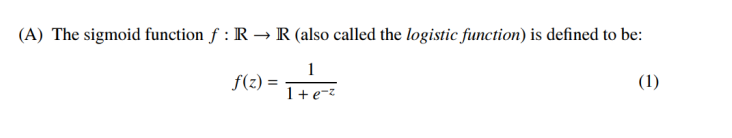
\includegraphics[width=6.49167in,height=1.84167in]{image6.png}\\
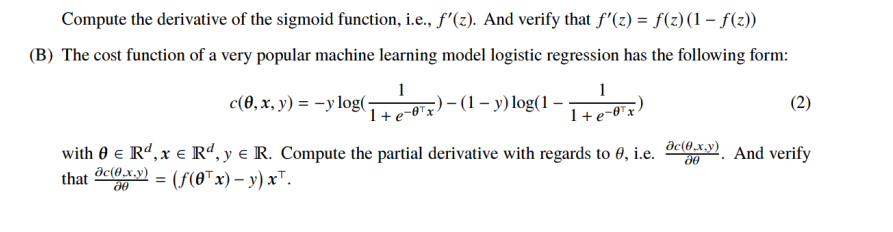
\includegraphics[width=6.49167in,height=1.84167in]{image7.png}\\

\emph{a)}



\[\frac{\partial f(z)}{\partial z} = \frac{e^{- z}}{{(1 + e^{- z})}^{2}} = \frac{1}{1 + e^{- z}}\left( 1 - \frac{1}{1 + e^{- z}} \right) = f(z)(1 - f\left( z \right))\]

\emph{b)}


\begin{center}
  \emph{..To be added..}
\end{center}


\textbf{Code implementation:} \href{https://colab.research.google.com/github/dtungpka/Applied-Mathematics-for-Artificial-Intelligence/blob/main/Assignment_3/Assignment%203.ipynb#scrollTo=Problem_6}{Problem 6}



\end{document}
